% arara: xelatex: {shell: true}
% arara: biber
% arara: xelatex: {shell: true}
% arara: xelatex: {shell: true}
\documentclass[letterpaper,10pt]{article}
\usepackage[margin=1in]{geometry}
\usepackage{hyperref}
\usepackage{datetime}
\usepackage{graphicx}
\usepackage[justification=centering,font=small,labelfont=bf]{caption}
\usepackage{fancyhdr}
\usepackage[backend=biber,
date=iso,
seconds=true,
style=numeric,
]{biblatex}
\addbibresource{canbusre.bib}

\pagestyle{fancy}
\rhead{DSSCAW Technical Report \#001}

\title{Give. Sympathize. Control.\\
Subverting the GZM48S Lawnmower via CAN\thanks{
 \href{https://www.dsscaw.com/}{Dirty South Supercomputing} on behalf of \href{https://www.greenzie.com/}{Greenzie} of Atlanta, GA.
}\\
}
\author{Nick Black, Consulting Scientist\\
\texttt{nickblack@linux.com}
}

%%%%%%%%%%%%%%%%%%%%%%%%%%%%%%%%%%%%%%%%%%%%%%%%%%%%%%%%%%%%%%%%%%%%%%%%
\begin{document}
%%%%%%%%%%%%%%%%%%%%%%%%%%%%%%%%%%%%%%%%%%%%%%%%%%%%%%%%%%%%%%%%%%%%%%%%
\date{2019-08-01}
\maketitle
\thispagestyle{fancy}
\begin{abstract}
I accessed the CAN (Controller Area Network) bus of the Greenworks Commercial
Stand-On Mower (GZM48S). This CAN network was sniffed as various controls were
manipulated. I analyzed the various CAN messages. I verified that, using my
derived model of the CAN network, messages injected into the CAN bus had
physical effects on the mower. I finally propose further steps necessary to
reliably and smoothly control the mower from a ROS software stack.
\end{abstract}
%%%%%%%%%%%%%%%%%%%%%%%%%%%%%%%%%%%%%%%%%%%%%%%%%%%%%%%%%%%%%%%%%%%%%%%%
\section{Introduction}
The GZM48S\parencite{gzm48s-owners}\parencite{gzm48s-parts} is an electric,
lithium-ion lawnmower designed for a standing human operator. Greenzie desires
to autonomously drive this mower using their ``Archer'' ROS\parencite{ros}
software stack. Rather than attempt to mechanically manipulate the human
controls, Dirty South Supercomputing was contracted to reverse engineer the
mower's CAN bus, and determine whether the mower can be operated via CAN
messages.

Sniffing the CAN bus revealed several dozen distinct CAN message IDs (CAN has
no concept of source or destination addresses, but all message types have a
unique 11- or 29-bit identifier). CAN IDs are not standardized across products,
but by correlating the message types with various mower behaviors, it was
possible to derive a consistent model of the message semantics. Various
messages were composed by hand and injected into the CAN bus, with results
including changes on the mower's LED, interruption of expected mower behaviors,
and faulting the mower (requiring a power cycle).

It was not possible to initiate or maintain most motor effects via injected CAN
messages, but this is explainable given the presence of CAN \textit{message
contention}\parencite{ogdynamite}. ECUs (Electronic Control Units, the various nodes on the CAN
network) typically broadcast their messages regularly, often dozens of time per
second. When a message ID periodically sent by some ECU is injected by our
stack, the ECU is likely to contradict that message within a short time (on the
order of milliseconds), too quickly for motors to reflect the momentary
engagement. It is not known whether this is the \textit{sole} obstacle to controlling
the motor with our stack{\textemdash}it is possible that further controls
restrict our CAN messages from controlling the motor and blades. A plan for
weapons-grade control is proposed, which I believe to be feasible.
\section{Setup}
The Greenworks Commercial GZM48S mower's
rear electrical area, when opened, reveals a male DE-9. This interface seems
wired according to \S6.1 of the CiA 303-1\parencite{cia3031} recommendation regarding
the ISO 11898-2\parencite{iso118982} CAN specification (``D-SUB 9-pin connector'').
The PEAK System PCAN-USB\parencite{pcan} IPEH-002022\footnote{This variant
includes a TLP291 optocoupler.} bridges a corresponding
female DE-9 to a USB 2.0 Type A, employing an NXP SJA1000\parencite{sja1000}
controller and an NXP PCA82C251\parencite{pca82c251} transceiver.
CAN buses are not guaranteed to be safe for hot-added
devices; it is advised to connect the PCAN to the bus only while the mower is
powered off\footnote{In practice, ensuring that GND is connected prior to
$V_{cc}$ should suffice.}.

\subsection{Host side}
The PCAN was connected to a Lenovo T580 laptop running a custom 5.1.3 Linux
kernel and Arch's version 2018.02.0-3 of the \textit{can-utils}\parencite{canutils}
tools\footnote{v2018.02.0 was current in both Arch and Debian Unstable at the time,
though commits have been made since then.}. It was recognized by the \texttt{peak\_usb}
kernel module, and verified as having the current firmware (version 8.4).
\texttt{peak\_usb} is a SocketCAN driver, and results in a network-style
device e.g. \texttt{can0}. This device requires, at minimum, timing
configuration. It was possible to sniff packets without registered errors using
the \texttt{bitrate 125000} parameter to \texttt{ip}, indicating the
CiA-recommended timing\parencite{canbittiming} for a 125kbit/s network\footnote{8$\mu$s nominal bit
time $t_B$, 16 quanta per bit, 625ns time quantum $t_q$, samplepoint at 14$t_q$
(7$\mu$s).}. At other rates (including 500 and 250kbit/s), we received only errors.

The following further options were applied to the interface:
\begin{itemize}
\item \texttt{restart-ms 1}: Renegotiate as quickly as possible if we enter
  the BUS-OFF error state.
\item \texttt{one-shot off}: Retransmit on ACK failure.
\item \texttt{berr-reporting on}: Enable error reporting IRQs.
\end{itemize}
We explicitly do \textit{not} use \texttt{triple-sampling on},
\texttt{listen-only on}, nor \texttt{fd on}. See the ``Questions'' section
regarding FD. A series of captures were acquired on-site the Saturdays of
2018-05-11 and 2018-05-18. The command used to generate the captures was:\\

\texttt{candump -ta -a -l -r\$((1024 * 1024 * 8)) -D -d -l can0,0:0,\#FFFFFFFF}\\

At least 500 packets were seen per second when the mower is powered on, rising
as high as the 600s. These logs can be replayed using \texttt{canplayer} either
onto a virtual CAN device (for analysis with e.g. \texttt{cansniffer}) or onto
a physical CAN interface for injection. They are most easily viewed as ASCII
text using \texttt{log2asc}. All three programs are distributed as part of
\textit{can-utils}. While the dump was running, interface state and statistics
were monitored using:\\

\texttt{watch -n2 ip -details -s l show can0}\\

It is important to watch both RX and TX errors, as well as the CAN controller's
error state\cite{canerrors}. A CAN controller can be in one of three error
states:
\begin{itemize}
\item ERROR-ACTIVE: The controller can transmit normally.
\item ERROR-PASSIVE: The controller must wait longer to transmit, and may not
  send active error frames.
\item BUS-OFF: A conforming device must not transmit until renegotiated.
\end{itemize}
While the \texttt{restart-ms 1} option will result in quick renegotiation, it
is undesirable to enter this state, and makes transmission impossible using most
devices. Note that these error-containment mechanisms can themselves be
exploited as a DoS attack\parencite{errorvulns}.

\subsection{Mower side}
With regards to the mower, we are most interested in the left and right steering
control lever (each can be independently placed in forward, backward, neutral,
or the parked default), and the pressure sensor underneath the operator's stand.
Without effort, both levers will spontaneously return to the disabled state,
and the platform will return to its original level. If any of these three inputs
are not engaged, the unmodified mower will not move. Of further interest are
the drive speed switch, the blade speed switch, and the blade engagement button.
All three retain whatever state they're placed in, and it is thus less critical
to manage them via the CAN bus.
\begin{center}
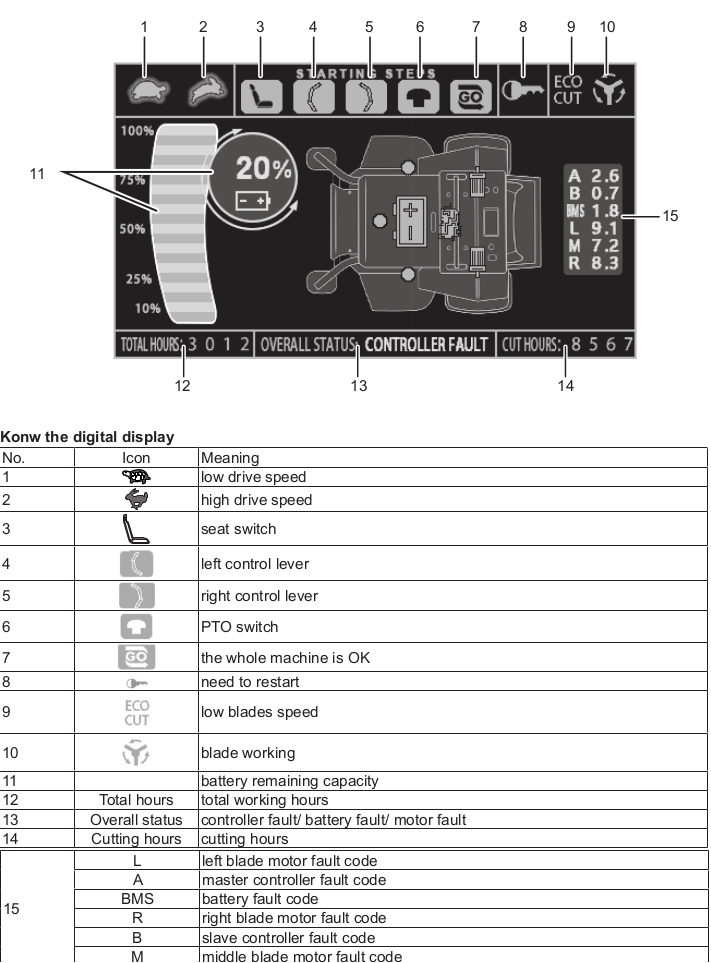
\includegraphics[width=.9\linewidth]{mowerdisplay.png}
\captionof{figure}{GZM48S display\parencite{gzm48s-owners}. ``Konw'' \textit{sic}.}
\end{center}
It is possible to send the controller into a fault state (indicated by illumination
of the key icon (8) above) by injecting CAN frames. If this occurs, the mower
must be power cycled using the key. It has not been determined whether this
condition can be worked around via CAN bus. There are several less critical
faults, unaccompanied by the key icon. Powering the mower on with the blade
button engaged will boot into a controller fault, as will disengaging the
pressure sensor while the mower is operating. The leftmost three icons of the
``starting steps'' (3--5 above) must be lit, or the mower will not move. The
fourth icon (6) must be lit, or engaging the blades button (``PTO switch'')
will not start the blades.

The Owner's Manual rewards a close inspection. The diagram and accompanying
text suggest presence of both a ``master'' and ``slave'' controller. The terms
could suggest a failover protocol at work. CAN itself is a multi-master
protocol, but the CiA's CANopen\parencite{cia301} higher-layer protocol does
have a concept of masters and slaves. Note that it is implied that the master
speaks to the BMS (Battery Management System) and deck\footnote{``Deck'' and
``blades'' are used in a weird metonymy throughout the manual.} motor
controllers, but that both the master and slave speak to the HPD. ``KSI''
pretty clearly means ``Key Switch Input'', but what's an HPD? Human
Protection Device? Searching for this term in a CAN/industrial context pulls
on a thread which unravels to suggest that our two drive controllers are Curtis
1234\parencite{curtis1234} AC Induction Motor Controllers, eventually confirmed
via visual inspection\footnote{The mysterious HPD means ``high pedal disable'',
copied word-for-word from a Curtis manual.}. The 1234 speaks CANopen, and can
be configured as a CANopen master or slave. Later use of the term ``CAN NMT''
would seem to refer to CANopen's Network Management Protocol, of which there is
no concept in raw CAN. Indeed, we find CANopen NMTs in the packet captures.
Realizing this was a critical step in making sense of some of the more complex
CAN frames. Always study the documentation!
\begin{center}
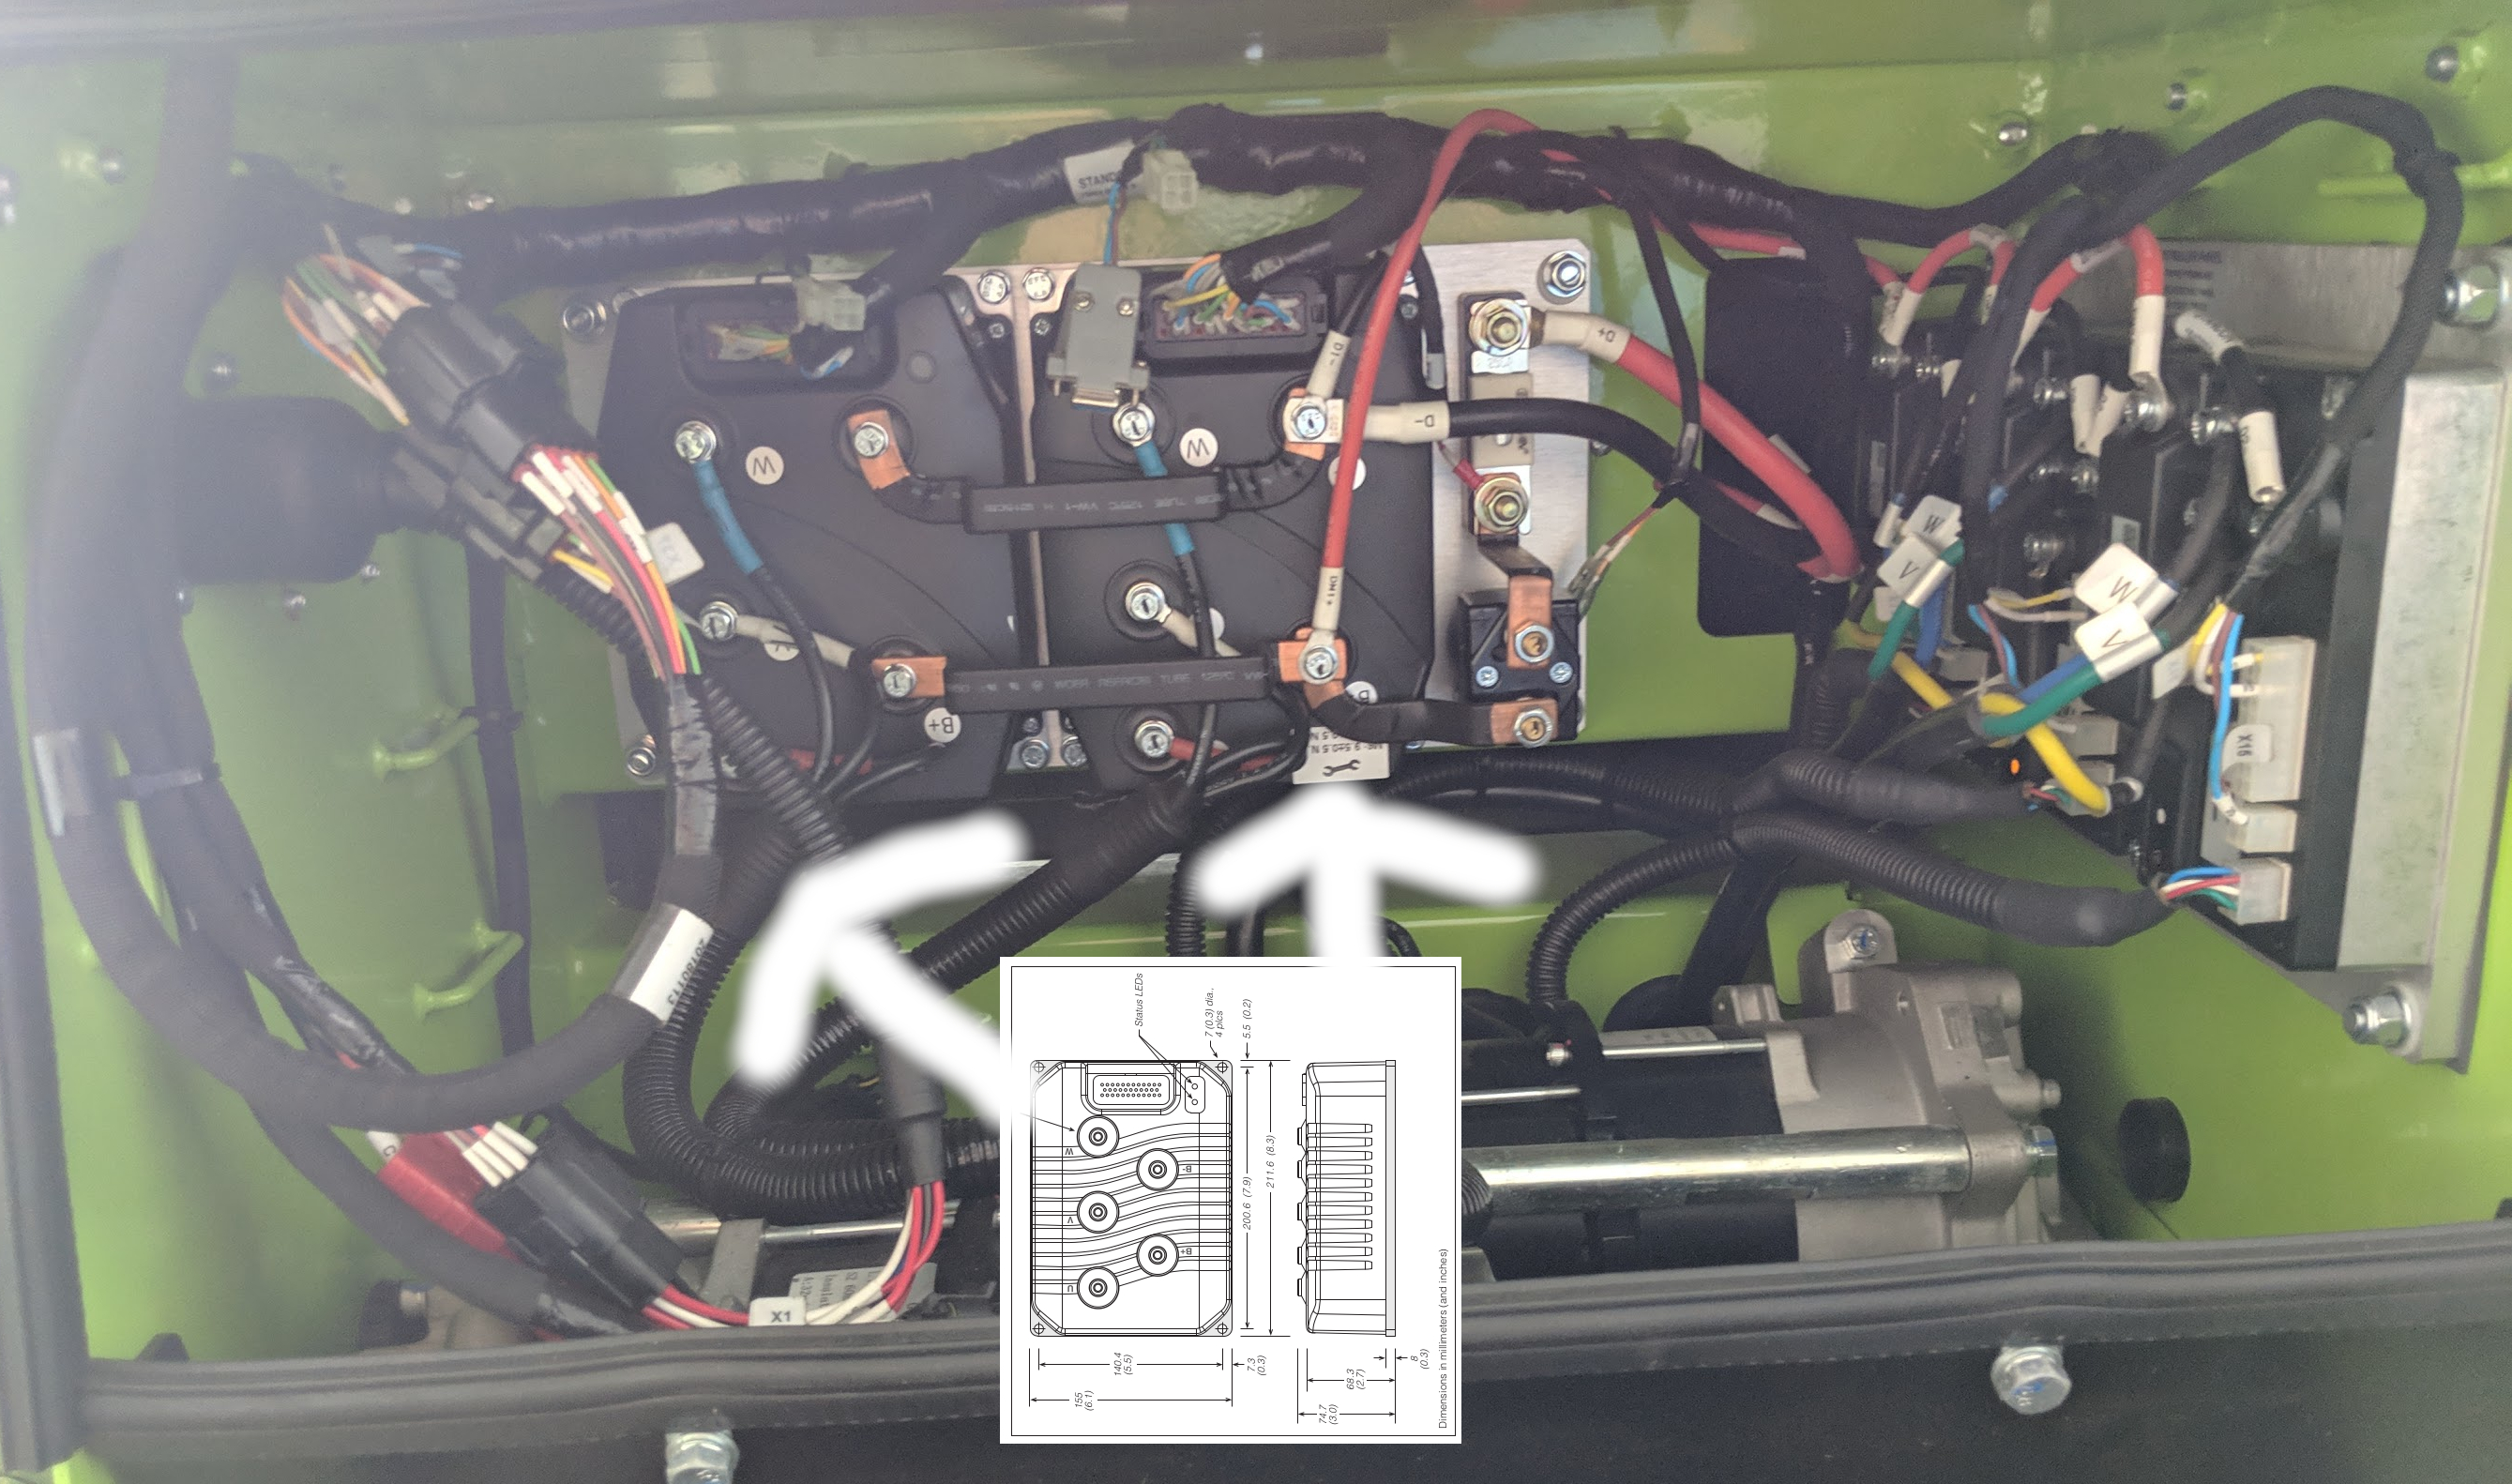
\includegraphics[width=.75\linewidth]{greenzie-electrics.jpg}
\captionof{figure}{GZM48S electrics bay, and diagram of Curtis 1234. It's a match!}
\end{center}

\section{Data and Interpretation}
As described above, traffic was captured using \texttt{candump}. It was then
analyzed using \texttt{cansniffer}, SavvyCAN\parencite{savvycan}, and bespoke
tools.
\subsection{CAN frames and semantics}
CAN is a minimalist link protocol. An 11-bit ID is mandatory, though modern CAN
networks support an extended 29-bit ID. This ID applies to a message \textit{type};
there is no concept of addressing in CAN. Logical 0 is \textit{dominant} over
the \textit{recessive} logical 1{\textemdash}if any node transmits 0 during a
bit, all nodes will see 0. Nodes must listen to the bus while transmitting, and
if they read a 0 while sending 1, must consider it a TX error. This does not
apply while transmitting the ID, which is near the head of the frame. In this
case, the node ought simply stop transmitting, and consider the bus arbitrated
away. Lower IDs thus have built-in priority over higher ones in a compliant
network. Each frame carries up to 8 bytes of payload. As noted earlier, there are
no ``well-known'' CAN IDs in the sense of e.g. TCP ports.

There is an element of support for single-message request-response in CAN, but
the vast majority of traffic tends to be unilateral broadcasting\footnote{A
request is a ``Remote Frame''. A broadcast{\textemdash}unilateral or
requested{\textemdash}is a ``Data Frame''.}. More generally relevant is
acknowledgement: towards the end of the frame is an ``ACK slot''. The
transmitter must transmit 1 for this bit, while listeners ought
transmit 0. If the transmitter does not read a 0, the message is unacknowledged,
and should be retransmitted. It is not generally possible to determine how many nodes on
the network ACKed the message, only that at least one did. It is finally important to
know that, upon encountering an error while in the ERROR-ACTIVE state, a node transmits
the Active Error Frame, which will collide with any ongoing message (prompting
a cascade of secondary error frames from other ERROR-ACTIVE nodes)\footnote{The
active error frame is 6 dominant bits followed by 8 recessive bits. Due to the
use of non-return-to-zero line coding with a length of 5, six clocks of 0 are
guaranteed to provoke the ``bit stuffing'' error on compliant, operating nodes.}.
\subsection{The GZM48S CAN bus}
The following 46 11-bit IDs were seen (not all were seen in all logs):

\begin{center}
\begin{tabular}[pos]{ | l | l | l | l | l | l | l | l | }
  \hline
ID & Len & ID & Len & ID & Len & ID & Len \\
  \hline
  1A6 & 8 & 1A8 & 8 & 1A9 & 8 & 1AA & 8 \\
  1AC & 8 & 224 & 8 & 225 & 8 & 226 & 8 \\
  228 & 8 & 229 & 8 & 22A & 8 & 22E & 8 \\
  2A6 & 8 & 2A8 & 4 & 2A9 & 4 & 2AA & 4 \\
  2AC & 8 & 301 & 8 & 302 & 8 & 303 & 8 \\
  304 & 8 & 305 & 8 & 306 & 8 & 307 & 8 \\
  308 & 8 & 320 & 8 & 321 & 8 & 326 & 8 \\
  350 & 8 & 351 & 8 & 352 & 8 & 353 & 8 \\
  354 & 8 & 355 & 8 & 3AC & 8 & 5A8 & 8 \\
  5A9 & 8 & 5AA & 8 & 628 & 8 & 629 & 8 \\
  62A & 8 & 726 & 1 & 727 & 1 & 728 & 1 \\
  \cline{5-8}
  729 & 1 & 72A & 1 \\
  \cline{1-4}
\end{tabular}
\end{center}

Already some patterns can be perceived. The same lower eight bits are seen in
many IDs{\textemdash}A8, A9, and AA show up together, as do 28, 29, and 2A. All frames
appear to have 8 bytes except for those prefixed with 7, which have 1 byte, and
some prefixed with 2, which have 4 bytes. Remember that higher IDs have lower
priority. Given that the lowest priority messages have only a single byte,
perhaps these are low-information heartbeats? Inspecting the 7xx frames
shows that they are all the same value (0x05), except upon boot. On boot,
they all show 0x7F. Together with a lack of any plausible prompting (why would
larger messages having higher priority be used to request such short ones?),
this could indeed possibly be either two request-response heartbeats, or four
unilateral ones.

\begin{center}
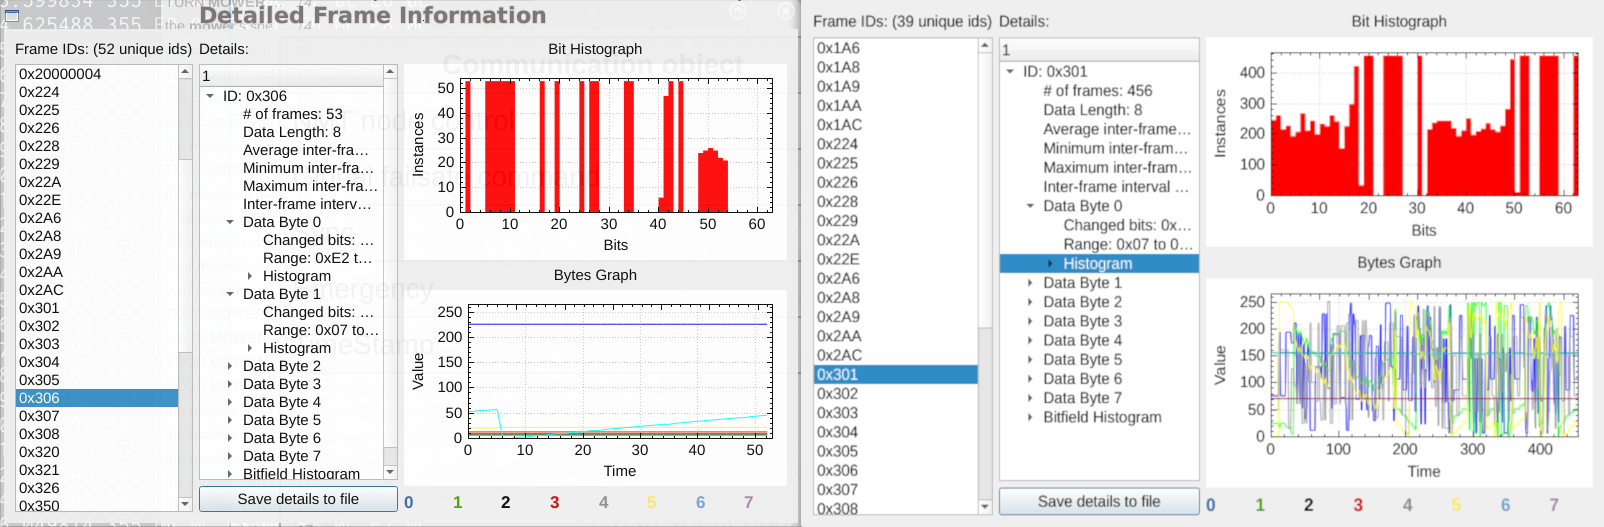
\includegraphics[width=.9\linewidth]{savvycan-dissimilar.png}
\captionof{figure}{Frame data analysis of two IDs using SavvyCAN.\\
What's going on in the left is pretty obvious. The right, not so much.}
\end{center}

In the case of 0x306, we see a lower-order byte rising in exact, visibly-recognizable
synchronization with time. When it reaches its maximum, it resets, and a higher-order
byte increases, yielding a fractal sawtooth. This can be nothing but a monotonically
increasing counter, and its wide domain suggests it to be a clock. We verify that
it is persistent across runs, and identify it as the source of ``total hours''.

\begin{center}
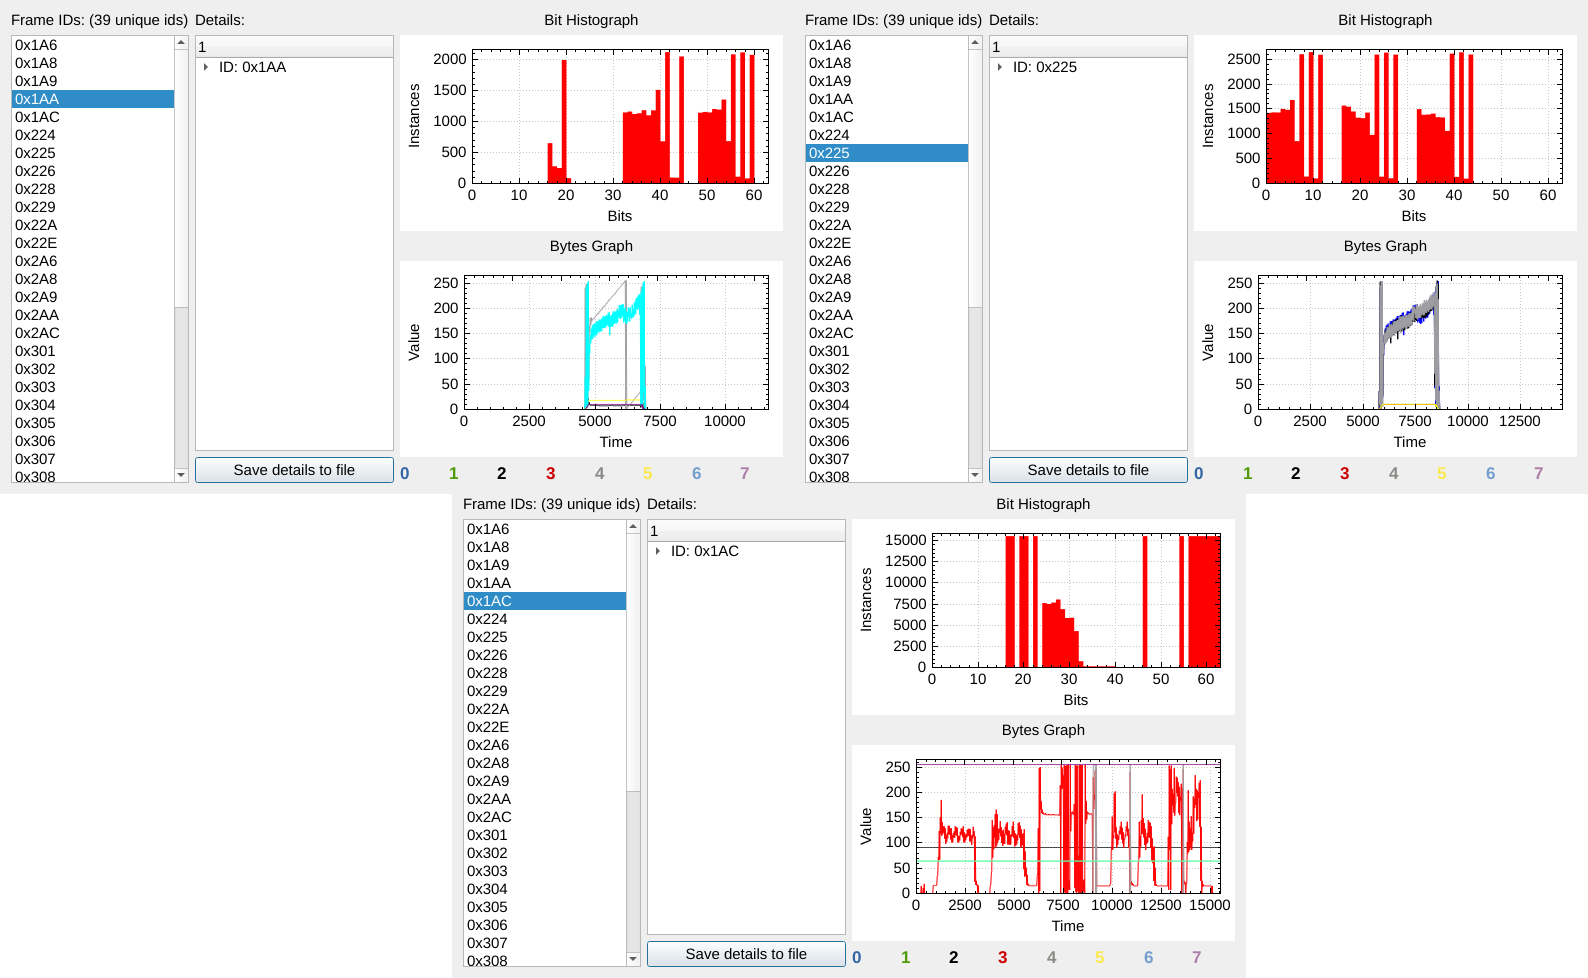
\includegraphics[width=.9\linewidth]{savvycan-related.png}
\captionof{figure}{Three IDs. Two are obviously correlated.\\
The bottom seems possibly to subsume the two on top, along with other data.}
\end{center}

During the first day's sniffing, the battery display indicated a 91\% charge.
The second day showed 90\%. These correspond to 0x5B and 0x5A, respectively.
In every frame having ID 224, the first byte is\ldots 0x5B on the first day,
and 0x5A on the second. Let's call it the human-readable battery level. This
suggests that 224 is either a message to the display, or a sensor message from
the BMS. It seems unlikely that the physical sensor would report a human-readable
value. It is determined that only the penultimate byte of 224 seems
otherwise to change, and it in very sharp, long-held changes among a few values,
usually in single-bit changes (e.g. 0xC to 0x4). This might plausibly be a
bitmask for the lights of the display. Could the other six bytes correspond to
the six error values? It's all reasonable, but by no means guaranteed.

The two analyses above involved sorting by ID and inspecting change among the
bytes of that ID's data frames. Stepping back, we sort by time, and plot all
the IDs, coloring them according to payload value:

\begin{center}
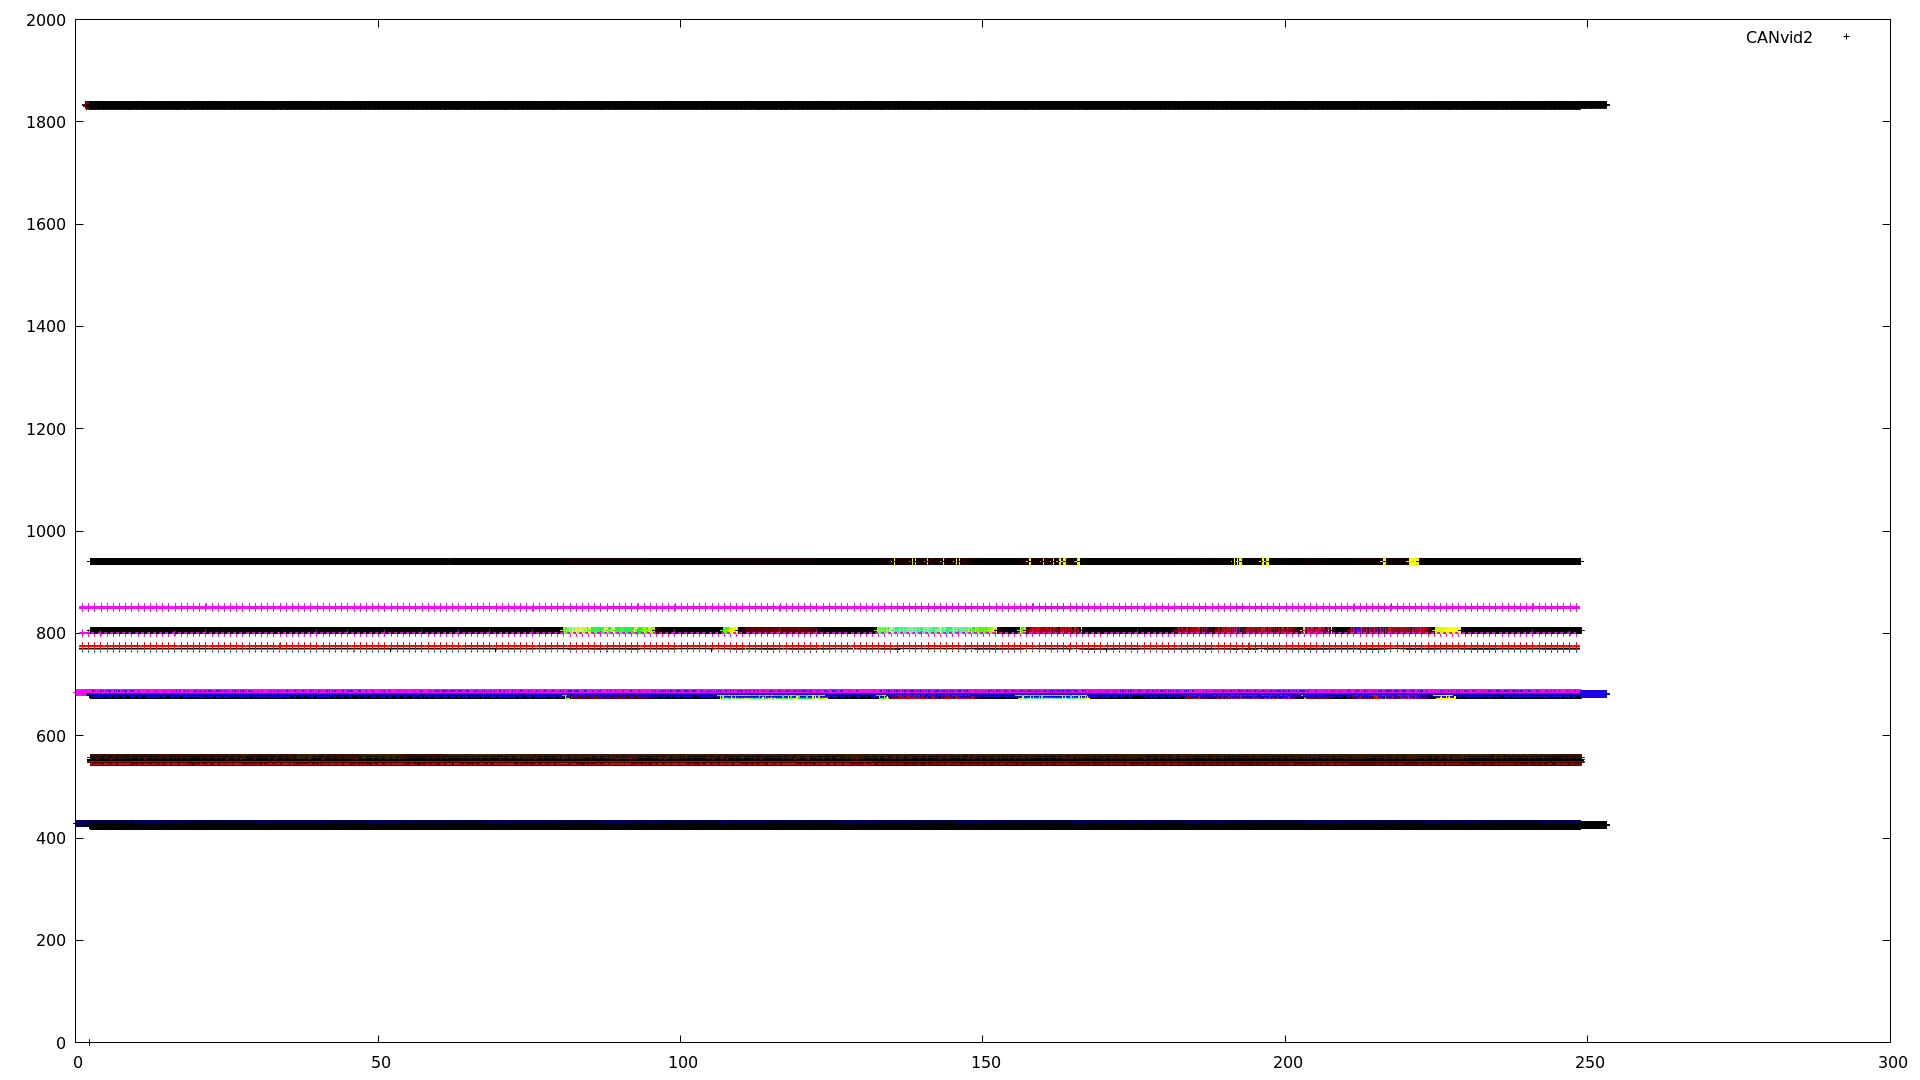
\includegraphics[width=.5\linewidth]{cantime.png}
\captionof{figure}{(Decimal) IDs over time, colored by payload.}
\end{center}

How many distinct nodes are responsible for these messages? We noted earlier
that the same lower 8 bits show up a few places. Assuming IDs
beginning with 1 to be inputs (hence low priority), I hoped to find a
correlation between e.g. 1A8, 1A9, 1AA and 2A8, 2A9, and 2AA. Alas, there is
none{\textemdash}but there most definitely exists one between 1A8, 1A9, 1AA and
228, 229, 22A! This difference of 0x80 is repeated in 5A8, 5A9, 5AA and 628,
629, and 6AA\ldots and in an ephiphany, we reach a new conjecture: the lower
\textbf{seven} bits could be node IDs, in which case 1A8, 228, 2A8, 5A8, 628,
and 728 are all a single node, 0x28. This unification would account for
essentially every ID save the 3xx series in just ten nodes. Inspecting the logs,
we do indeed see tight association between e.g. 1A6 and 226, and 2A6 and 326.
This interpretation grows more and more compelling.

\begin{center}
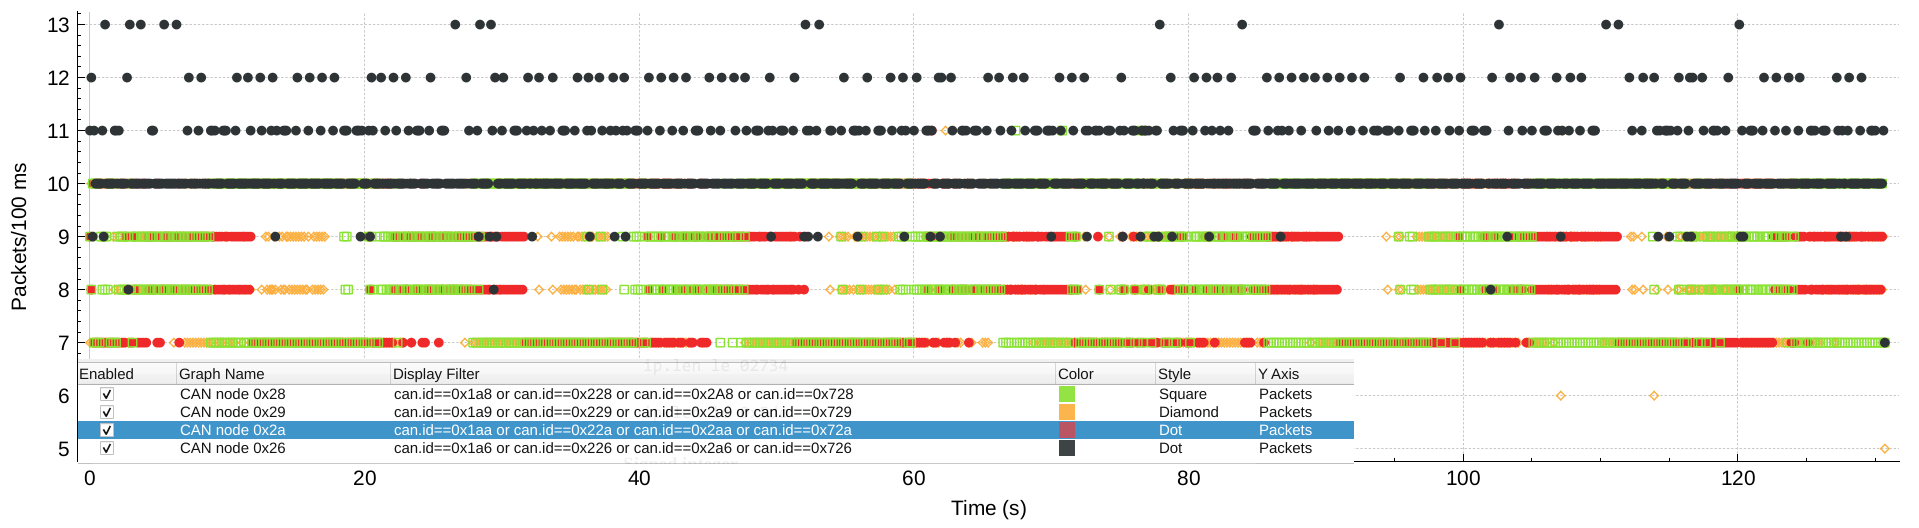
\includegraphics[width=1\linewidth]{wireshark.png}
\captionof{figure}{Wireshark I/O plot of four conjectured nodes.}
\end{center}

At this point, we have enough information to consult known higher-level
protocols. As mentioned earlier, the term ``NMT'' is used once in the manual,
copied from the Curtis 1234 error descriptions. This could be CANopen (which
is indeed supported by the Curtis unit), with its Predefined Connection Set:

\begin{center}
\begin{tabular}[pos]{ | l | l | l | l | }
  \hline
Message	& Function code	& CAN-ID base & COB-ID parameter index \\
  \hline
NMT	& 0000 & 000 & Not configurable \\
SYNC & 0001	& 080 & 1005 \\
EMCY & 0001	& 081--0FF & 1014 \\
TIME & 0010	& 100 &	1012 \\
$\mathrm{TPDO_1}$ & 0011 &	181--1FF & 1800 \\
$\mathrm{RPDO_1}$ & 0100 & 201--27F & 1400 \\
$\mathrm{TPDO_2}$ & 0101 & 281--2FF & 1801 \\
$\mathrm{RPDO_2}$ & 0110 & 301--37F & 1401 \\
$\mathrm{TPDO_3}$ & 0111 & 381--3FF & 1802 \\
$\mathrm{RPDO_3}$ & 1000 & 401--47F & 1402 \\
$\mathrm{TPDO_4}$ & 1001 & 481--4FF & 1803 \\
$\mathrm{RPDO_4}$ & 1010 & 501--57F & 1403 \\
TSDO & 1011 & 581--5FF & Not configurable \\
RSDO & 1100 & 601--57F & Not configurable \\
Heartbeat	& 1110 &	701--77F & Not configurable \\
  \hline
\end{tabular}
\end{center}

It seems safe to proceed under the assumption that CANopen is in play. We
replay the \texttt{candump} log over a virtual CAN interface\footnote{Use the
Linux \texttt{vcan} module.}, and capture it in Wireshark\parencite{wireshark},
applying its CANopen secondary decoder. The various frames all decode into
reasonable CANopen, and a node table emerges:

\begin{center}
\begin{tabular}[pos]{ | l | l | l | l | l | l | l | l | l | }
  \hline
%Node & TP1 & RP1 & TP2 & RP2 & TP3 & NMT & TS & RS \\
Node & TPDO1 & RPDO1 & TPDO2 & RPDO2 & TPDO3 & NMT & TSDO & RSDO \\
  \hline
0x26 & 1A6 & 226 & 2A6 & 326 & & 726 & & \\
0x27 & & & & & & 727 & & \\
0x28 & 1A8 & 228 & 2A8 & & & 728 & 5A8 & 628 \\
0x29 & 1A9 & 229 & 2A9 & & & 729 & 5A9 & 629 \\
0x2A & 1AA & 22A & 2AA & & & 72A & 5AA & 62A \\
  \hline
\end{tabular}
\end{center}
%0x01 & & & & 301 & & & & \\
%0x02 & & & & 302 & & & & \\
%0x03 & & & & 303 & & & & \\
%0x04 & & & & 304 & & & & \\
%0x05 & & & & 305 & & & & \\
%0x06 & & & & 306 & & & & \\
%0x07 & & & & 307 & & & & \\
%0x08 & & & & 308 & & & & \\
%0x20 & & & & 320 & & & & \\
%0x21 & & & & 321 & & & & \\
%0x24 & & 224 & & & & & & \\
%0x25 & & 225 & & & & & & \\
%0x2C & 1AC & & 2AC & & 3AC & & & \\
%0x2E & & 22E & & & & & & \\
%0x50 & & & & 350 & & & & \\
%0x51 & & & & 351 & & & & \\
%0x52 & & & & 352 & & & & \\
%0x53 & & & & 353 & & & & \\
%0x54 & & & & 354 & & & & \\
%0x55 & & & & 355 & & & & \\
TPDOs 0x2A8, 0x2A9, and 0x2A are responsible for the 4-byte messages. All other
messages, save the single-byte 0x7xx-series heartbeats, are 8 bytes. It seems
reasonable to assume that these three nodes{\textemdash}0x28, 0x29, and
0x2A{\textemdash}are a logical group, and indeed they are almost certainly the
three blade controllers (see the right side of Figure 2). Their activity takes
a distinctly different form when the blades are engaged, and the SDO messages
to and from these nodes are (sometimes, but only) sent immediately prior to
blades turning on. Analysis of the NMT state machine and the 7xx messages
confirms this, and further implies 0x26 and 0x27 to be a group. It's almost
certain that these are the Curtis drive controllers, and examining the changes
in TPDOs 0x1A6 and 0x2A6 confirms a strong correlation with mower movement.

The changes in 0x224, as noted earlier, seem to cover the gamut of state
changes, and can be put on an isomorphism with display changes.  The first
two bytes are a human readable battery level. The seventh byte is a bitmask
corresponding to the top row's icons (save the key icon, and with a sole bit
to choose between the mutually exclusive low and high speed glyphs). The other
six bytes probably carry the six error codes. The two hour counts correspond
to four bytes of the clock signal at node 0x06.

If the motor controllers are to be driven through CAN in their current
configuration, I suspect that it would be via RPDO 226 and 326, but I cannot
isolate a control signal on these IDs. Nor can I correlate any other signal
to the drive levers. Examining its manual, the Curtis 1234 does not appear, by
default, to use CAN bus as an input, but rather the various throttle and brake
pot inputs. CAN is instead being used to report motor state, including level
and temperature. The Curtis 1234 supports uploading firmware written in 
Vehicle Control Language, and it is probable that CAN could be used as a control
input with a custom firmware. It would likely be easier, however, to drive the
input lines from the Archer system. It \textit{does} seem likely that the
blade controllers are set up for driving with CAN, due to the exchange of SDO
messages. As noted above, however, this does not always happen upon blade
engagement.

\section{Replay experiments}
I injected CAN frames via two different strategies: bulk replay of recorded
traffic, and surgical injection of packets constructed according to the analysis
above.

Traffic sniffed while standing on the pressure sensor, replayed while not
standing on the sensor, did indeed cause the display to illuminate the stand
light. The light flickered, presumably due to contradictory messages being
interleaved with the replayed messages. At no time did the mower begin moving,
despite the traffic being sniffed while moving. This is almost certainly due
to the KSI system being hard-wired to the motor controllers (it has distinct
wired inputs), and said controllers synthesizing these values on 224 outputs.
I then dropped all but the 224 messages from this traffic, and repeated the
experiment. The same results were seen.

Traffic sniffed while \textit{not} standing on the pressure sensor was then
replayed while standing on the mower with the levers in park, leading to the
sensor light flickering. This was again due to RPDO 224. I began driving the
mower forward, and played this traffic back once more. The light flickered,
and the mower stuttered, but no recoverable controller fault (as occurs when
one jumps off the stand while moving) was seen. This latter lends credence to the
idea that the display is controlled by CAN, but the motor controls are not.
The stuttering of the mower, however, would seem to suggest otherwise. It is
possible that we were momentarily stopping the motor, but that ought have led
to a safety fault; I instead believe that dumping so much traffic onto the CAN
bus (the messages were injected in a tight loop) simply upset the controllers.
Certainly I was unable to cause a sedentary mower to move, however
stutteringly.

Sending enough traffic, of any kind, eventually led to non-recoverable
controller faults, likely due to drowning out of important messages (including
heartbeats).

\section{Towards control}
The following facts are now known:
\begin{itemize}
\item CAN frames can be sniffed from the DE-9 port, and these CAN frames can
      be consistently correlated with mower operation.
\item CAN frames injected via the DE-9 port can result in changes to the mower's
      display, including turning on lights indicating control engagement. Of the
      four lights necessary to trigger the mower's ``GO'' light, all four
      (stand pressure, left control, right control, blades enabled) can be
      illuminated by CAN frame injection.
\item CAN frames injected via the DE-9 port can result in degraded mower,
      functionality, including disabling blades and retarding movement.
\item CAN frames injected via the DE-9 port can fault the mower, requiring a
      restart. A restart requires at least 5 seconds.
\end{itemize}

No concrete mapping of CAN traffic to desired mower behavior has been found.
That doesn't mean that none exists. Aside from simply overlooking a signal,
the following are all possible:
\begin{itemize}
\item Contradictory messages{\textemdash}message contention{\textemdash} could
  be invalidating our constructed controls. This would mean I've misidentified
  an input as an output, and that the Curtis controllers have been reprogrammed
  for CAN control, in a way that would seem to require custom VCL. If this is
  true, working around the issue would require either disconnecting the true
  CAN input (electrically or via DoS), timing our messages to arrive precisely
  after that input (plus luck{\textemdash}it's in no way certain that this
  would result in deired behavior), or invalidating each broadcasted input.
\item My injected messages are being filtered from the controllers (but not
  from the display, which we can affect).
\item CAN controls are checked against the electromechanical inputs, and
  ignored if they're clearly incompatible (very likely for e.g. safety systems).
\end{itemize}

If my conjectured control messages are indeed correct (I do not think that
they are; I believe them to be outputs, not inputs), and their failure is due
to contention, it ought be possible to disconnect the conflicting controls,
and see them work. I do not expect this line to succeed after reading the
Curtis manuals and running my tests.

I see no means for our messages to be filtered from the drive controllers, but
not filtered from the display. This would seem to require two distinct CAN
buses, with a filtering bridge in the middle. I see no indication of such a
device, and again, this is predicated on the controls being correct in the first
place. If they are correct, but being checked against electomechanical inputs,
it seems unlikely that the supposed CAN controls would work in the absence of
said inputs, meaning they'd need be controlled in any case.

I thus recommend that efforts to drive the GZM48S focus on using the Curtis
controllers' non-CAN inputs. These interfaces are fully documented, and known
to work. If driven by the Archer stack, there exist no other controls to
compete with our operation. A less appealing option is to write new VCL for the
controllers, and upload it using a 1311 programmer, an operation too far
removed from my skill set for meaningful comment.

On the plus side, should such control be put into place, the sensor signals
emitted in the CAN network now seem well understood, and can be used by our
system.

\section{Questions}
\begin{itemize}
\item The PCAN-USB manual claims that soldering is required to effect the
  necessary 120$\Omega$ termination for Hi-Speed CAN (ISO 11898-2), or a
  PCAN-TJA1054 bus converter for Lo-Speed CAN (ISO 11898-3)\parencite{iso118983}.
  Neither of these options were used. The PCAN appeared to work fine with the
  network at 125kbit/s. Is this correct, or are we missing something?
\item The created network device's MTU is 16, not the 72 expected from
  FD-capable CAN. Are we possibly missing CAN FD messages? It might be best to
  test with \href{PCAN-View}{https://www.peak-system.com/PCAN-View.242.0.html}.
\item I did not attempt to scan or otherwise interrogate the ECUs using e.g.
  the ODB-II diagnostic protocol. Might there be things waiting, listening?
\end{itemize}
%%%%%%%%%%%%%%%%%%%%%%%%%%%%%%%%%%%%%%%%%%%%%%%%%%%%%%%%%%%%%%%%%%%%%%%%
\printbibliography
\end{document}
